\chapter{Risultati Sperimentali}
\label{chap:Risultati sperimentali}

\section{Addestramento}
\label{sec:Addestramento}

Il modello è stato addestrato utilizzando la tecnica della \textit{cross-validation} (vedi Figura
\ref{fig:cross_validation}), con una suddivisione dei dati in cinque parti uguali (cinque folds). In
questo contesto di apprendimento supervisionato, al modello sono state fornite immagini originali
insieme alle loro corrispondenti segmentazioni effettuate manualmente.

\begin{figure}[!ht]
    \centering
    \includegraphics[width=0.7\columnwidth]{Immagini/training.png}
    \caption{Processo di addestramento del modello}
    \label{fig:addestramento_del_modello}
\end{figure}

L'addestramento è stato eseguito per 5 iterazioni, utilizzando un fold diverso in ciascuna
iterazione. L'errore finale è stato calcolato come la media degli errori ottenuti in ciascuna delle
cinque iterazioni.


\begin{figure}[!ht]
    \centering
    \includegraphics[width=0.4\columnwidth]{Immagini/fold_0_loss.png} \includegraphics[width=0.4\columnwidth]{Immagini/fold_0_accuracy.png}
    \caption{Errore e accuratezza della prima porzione di dati}
    \label{fig:loss e accuratezza della prima porzione di dati}
\end{figure}

\begin{figure}
    \centering
    \includegraphics[width=0.4\columnwidth]{Immagini/fold_1_loss.png} \includegraphics[width=0.4\columnwidth]{Immagini/fold_1_accuracy.png}
    \caption{Errore e accuratezza della seconda porzione di dati}
    \label{fig:loss e accuratezza della seconda porzione di dati}
\end{figure}

\begin{figure}
    \centering
    \includegraphics[width=0.4\columnwidth]{Immagini/fold_2_loss.png} \includegraphics[width=0.4\columnwidth]{Immagini/fold_2_accuracy.png}
    \caption{Errore e accuratezza della terza porzione di dati}
    \label{fig:loss e accuratezza della terza porzione di dati}
\end{figure}

\begin{figure}
    \centering
    \includegraphics[width=0.4\columnwidth]{Immagini/fold_3_loss.png} \includegraphics[width=0.4\columnwidth]{Immagini/fold_3_accuracy.png}
    \caption{Errore e accuratezza della quarta porzione di dati}
    \label{fig:loss e accuratezza della quarta porzione di dati}
\end{figure}

\begin{figure}
    \centering
    \includegraphics[width=0.4\columnwidth]{Immagini/fold_4_loss.png} \includegraphics[width=0.4\columnwidth]{Immagini/fold_4_accuracy.png}
    \caption{Errore e accuratezza della quinta porzione di dati}
    \label{fig:loss e accuratezza della quinta porzione di dati}
\end{figure}


L'\textbf{errore} complessivo è stato calcolato come media degli errori ottenuti in ciascuna delle
cinque iterazioni di addestramento, utilizzando la formula \ref{eq:dice_bce_loss_complete}. Il
risultato è un errore medio del \textbf{$7.9\%$}.

Parallelamente, l'\textbf{accuratezza} complessiva è stata calcolata come la media delle accuratezze
ottenute in ciascuna iterazione, impiegando la formula \ref{eq:iou}. Ciò ha portato a un'accuratezza
media del \textbf{$92.1\%$}.

Oltre alle analisi quantitative, è stato fondamentale condurre analisi qualitative sulla
segmentazione ottenuta dal modello, specialmente considerando il suo impiego in ambito medico per la
segmentazione dei femori.

Nelle immagini seguenti viene riportato uno delle immagini prese in considerazione per
l'addestramento del modello e vengono mostrate le segmentazione manuali, le segmentazioni ottenute
dal modello e la differenze nella classificazione dei pixel tra le due segmentazioni.


\begin{figure}[!ht]
    \centering
    \includegraphics[width=0.7\columnwidth]{Immagini/image.png}
    \caption{Immagine originale}
    \label{fig:immagine originale}
\end{figure}


\begin{figure}[!ht]
    \centering
    \begin{minipage}{0.4\columnwidth}
        \centering
        \includegraphics[width=\linewidth]{Immagini/mask.png}
        \caption{Segmentazione manuale}
        \label{fig:segmentazione manuale}
    \end{minipage}
    \hfill
    \begin{minipage}{0.4\columnwidth}
        \centering
        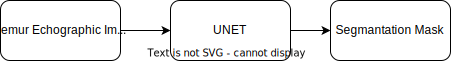
\includegraphics[width=\linewidth]{Immagini/prediction.png}
        \caption{Segmentazione del modello}
        \label{fig:segmentazione del modello}
    \end{minipage}
\end{figure}

% Per sostenere la tesi che il modello riesca a segmentare correttamente le immagini, \`e stata
% calcolata la distribuzione dei pixel per confrontare la segmentazione manuale con quella del
% modello.

Per confermare l'efficacia del modello nella segmentazione delle immagini, si è proceduto con
l'analisi della distribuzione dei pixel. Questa analisi confronta direttamente la segmentazione
manuale con quella ottenuta dal modello. L'obiettivo è dimostrare che la distribuzione dei pixel
nelle segmentazioni del modello corrisponde strettamente a quella delle segmentazioni manuali,
indicando così una segmentazione accurata.

\begin{figure}[!ht]
    \centering
    \begin{minipage}{0.45\columnwidth}
        \centering
        \includegraphics[width=\linewidth]{Immagini/handmade_scaled_hist.png}
        \caption{Distribuzione Intensità dei pixel della segmentazione manuale}
        \label{fig:distribuzione intensità dei pixel della segmentazione manuale}
    \end{minipage}
    \hfill
    \begin{minipage}{0.45\columnwidth}
        \centering
        \includegraphics[width=\linewidth]{Immagini/model_scaled_hist.png}
        \caption{Distribuzione Intensità dei pixel della segmentazione del modello}
        \label{fig:distribuzione intensità dei pixel della segmentazione del modello}
    \end{minipage}
\end{figure}

\begin{figure}[!ht]
    \centering
    \includegraphics[width=0.7\columnwidth]{Immagini/handmade_vs_model_scaled.png}
    \caption{Confronto tra la segmentazione manuale e quella del modello}
    \label{fig:confronto tra la segmentazione manuale e quella del modello}
\end{figure}

I risultati mostrano che la distribuzione dei pixel nelle segmentazioni generate dal modello si
allinea strettamente a quella delle segmentazioni manuali, suggerendo che il modello è in grado di
segmentare le immagini con precisione.


Dall'analisi dei risultati sia qualitativi che quantitativi, emerge che il modello mostra una
performance molto promettente. In particolare, si evidenzia che il modello supera abbondantemente
un'accuratezza del $90\%$, offrendo un ampio margine per ulteriori miglioramenti attraverso
l'incremento del numero di immagini disponibili per l'addestramento.

Degno di nota è la mancanza di ulteriori segmentazioni, non è necessario effettuare ulteriori
segmentazioni manuali per espandere il set di addestramento. Le nuove immagini raccolte possono
essere segmentate automaticamente utilizzando il modello e poi impiegate per rafforzare
ulteriormente il processo di addestramento. Questo approccio non solo semplifica il processo di
raccolta dati, ma accelera anche la possibilità di miglioramento e adattamento del modello a nuovi
dati.

